\chapter{Anomaly Detection Methods}
Detecting and exploring of anomalies in time series is a very important aspect, especially when dealing with power consumption data of physical infrastructure. Abnormal behavior is defined as a difference from the expected normal pattern. We use the terms abnormal behavior, anomalies and outliers interchangebly referring to same definition of unusual data pattern. We introduce two methods of anomaly detection, both methods assume a daily power usage pattern which, of course, can be different for each day of the week. Both techniques are not limited to daily patterns, but can be easily adapted to the periodicity of the underlying data set. The first described method is based on a weighted prediction, where recent measurements have a higher impact than older measurements \cite{janetzko2014anomaly}. The latter approach is transforming the observed daily pattern in the frequency domain and looking for dissimilarity in a transformed space.
\\

\subsection*{PCA-Based Anomaly Detection}
\textbf{PCA}

Due to the high dimensionality nature of our dataset, we consider Principal Component Analysis(PCA) as one of the anomaly detection technique in our work. PCA is used to transform the high dimensionality datasets into low dimensional dataset. This low dimensional dataset captures all the necessary features by capturing the required variance which can be used to study the patterns exhibited by our data. Mathematically, PCA is an orthogonal linear transformation that transforms the data to new axes such that the first principal axes captures the greatest variance after projecting the data into this new axes, the second axes captures the second greatest variance, third axes the third greatest variance and so on. These axes are called the principal axes or the principal components(PCs). The principal components are ordered by the amount of variance that they capture. It is considered one of the reliable methods in capturing the correlation between the datasets. This descriptive method has been developed for the detection of linear relations between variables. However, if the relationships between the variables analyzed are not linear, the values ​​of correlation coefficients can be  lower. 
	We consider normalizing our data before applying the PCA mainly because our data contains measures of different quantities such as voltages, current, power which are measured on different units. Normalizing the data is very essential preprocessing step before doing PCA, as the unnormalized data may lead to case where in each PC is dominated by a single variable. This would result in considering only one PC which has the largest variance and the remaining capturing very less variance.  In effect the results of the analysis will depend on what units of measurement are used to measure each variable. That would mean that principal component analysis should be done on raw data when all the measurements of our data are of same unit, which in turn will give more analysis weight on the variables which have higher variances. Therefore we standardize our data to mean equal to zero and standard deviation equal to one i.e $\mu = 0 ,  \sigma = 1 $. Standardizing the features so that they are centered around 0 with a standard deviation of 1 is not only important if we are comparing measurements that have different units, but it is also a general requirement for many machine learning algorithms.

\textbf{PCA for Anomaly Detection:} 

Our set of electrical data collected from the smart grids contains many features. Considering all these features together can make our anomaly detection process complex. We therefore divide our dataset by constructing two subspaces based on the variances contributed by the features into normal subspace and residual subspace. Normal subspace contains most of the variance in the data as captured by the first 'K' principal components. Residual subspace is constructed by the remaining N-K components which contains very less variance in the data. The number of principal components(k) to choose will be discussed further in this section. Consider our data set containing $i$ observations(rows) and $j$ features(columns) which can be represented as a data matrix Y, so Y is a $i * j$ matrix. Each observation contains j features and denoted by single data point. From now on whenever we say a data point it represents $i$-th row containing j features of the data matrix Y.
\begin{figure}[tph!]
\centerline{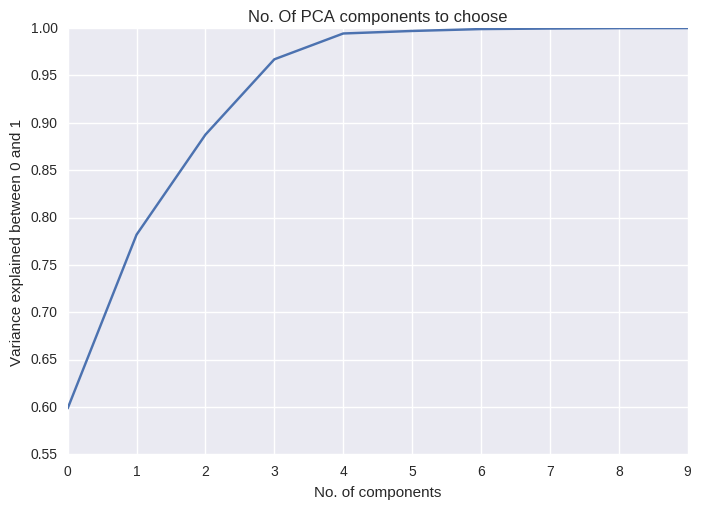
\includegraphics[totalheight=6cm]{PCA_number_of_elements_to_choose.png}}
    \caption{PCA Components}
    \label{fig:verticalcell}
\end{figure}

\subsection*{Prediction-Based Anomaly Detection}
The basis for prediction is an observed pattern and the assumption that it is reoccurring (with slight modifications) in the future. We assume our data follows a regular underlying pattern
and therefore also assume that the model describes the usual behavior well. Detecting anomalies using prediction follows this idea and is related to the statistical measure of residuals. Basically, this method predicts a value for each minute of the day by taking all previous measurement at the same time of the day. As an example, assume we predict the value for a Tuesday at 11:05am. We would now average all previous observed values of a Tuesday at 11:05am. Taking just an average would have the disadvantage of neglecting recent developments in the time series \cite{janetzko2014anomaly}. We therefore use a weighted averaging scheme with higher factors for recent values and linearly decreasing influence weights for older values. Further detailed explanations can be found in \cite{hao2011visual}.

After predicting for each point in a time series the expected values based on all values occurring before this point in the time series, we can compute the difference between predicted and observed values. The difference is an indicator for the abnormality of the point in a time series but needs for higher expressiveness some kind of normalization. From the choice and the design of the prediction method we are assuming a model which may not be applicable to all observed time series. We counterbalance for this fact by calculating the average fitting of our model. More in detail, we compute the average deviation from the predicted values for the whole time series. If a whole time series is highly unpredictable, the differences between predicted and actual values are less meaningful compared to a case when a time series follows perfect daily patterns with small deviations. Computation of the anomaly score is summarized by the following equation \cite{janetzko2014anomaly}:

anomaly[time] = $\frac{|predVal[time] - obsVal[time]|}{avgt∈Time (|predVal[t] - obsVal[t]|)}$\\

\subsection*{Clustering-Based Anomaly Detection}
\frenchspacing
The second approach for detecting anomalies in time series data is similarity-based. We assume often-observed patterns to be the usual behavior and rarely occurring patterns to be abnormal. Following this idea, we first have to define and compute the similarity of patterns in order to detect whether a pattern occurs more than once. The approach described in this section is proposed and presented by Bellala et al. in [\cite{bellala2012following},\cite{bellala2011towards}]. The time series is first partitioned into days and afterwards transformed by a Fourier transformation into the frequency domain. Each day of the time series is resulting in a k-dimensional vector in the frequency domain with k being a parameter of the transformation process. The next step described by Bellala et al. is a dimension reduction by multi-dimensional scaling into a two-dimensional space. The density distribution in the reduced MDS space is now interpreted as an anomaly score. Points (time series of a single day) being in a high-density area with many (similar) neighbors are assumed to reflect the usual behavior. Outliers in the 2D space can be seen as days with unusual values and are assigned a high anomaly score. This technique only takes the frequency domain into account and does not integrate external effects like weather data or week of the day.\\

 \subsection*{Gaussian Mixture Model-Based Anomaly Detection}
Here we propose yet another unsupervised algorithm for anomaly detection using Gaussian Mixture Model. The Gaussian Mixture Model(GMM) is used to model the probability density function of a feature vector, x, by the weighted combination of M multi-variate Gaussian densities $(\lambda)$ \cite{marinai2007machine} :
\begin{equation}\label{eq:1}
  p(x|\lambda)= \sum_{i=1}^{M} {p_ig_i(x)}  \\
 \end{equation}

First we fit a Gaussian Mixture Model (GMM) with Gaussians centered at each data point to a given data set. We then estimate the mixture proportion by applying Expectation Maximization algorithm to the given dataset. Each mixture proportion will represent the degree to which the point is a cluster center. The higher the mixture proportion, the more likely it is a cluster center, which means it has higher influence on other points. Reversely, the lower the mixture proportion is, the less likely the point is a cluster center, which means it has lower influence on other points. The outlier factor at each data point is then defined as a weighted sum of the mixture proportions with weights representing the similarities to other data points.	

\begin{figure}[tph!]
\centerline{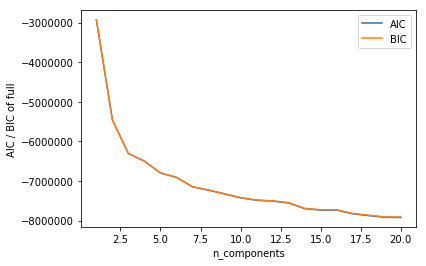
\includegraphics[totalheight=6cm]{BIC_1.png}}
    \caption{BIC score to determine the number of gaussians to choose}
    \label{fig:verticalcell}
\end{figure}
\label{sec:Algorithm}

Given a set of data points$ X ={x_1, . . . , x_n} $, a standard Gaussian mixture model clustering seeks to maximize the scaled log-likelihood function \cite{perl2009outlier}\\
\begin{equation}\label{eq:2}
  l(\pi_{1:m}, \mu_{1:m}, \lambda; X)= \frac{1}{n}\sum_{i=1}^{n} {log[\sum_{j=1}^{m}{\pi_ jp(x_i|\mu_j,\lambda)}]}  \\
 \end{equation}
 where m is the number of model components, $\pi_j = p(\omega_j |\lambda)$ represents the strength of jth component $\omega_j$ with $\sum_{i=1}^{m}{\pi_i = 1}$ and $\pi_{1:m}$ is a vector composed of $\pi_j$ for j = 1, . . . , m. The probability $p(x_i|\mu_j , \lambda)$ is a Gaussian and $\lambda$ is a vector of parameters specified below.

In the standard mixture model $\mu_j$ is the unknown mean vector for jth component and is estimated together with other parameters using an EM algorithm. Since our goal is not clustering but an estimation of an outlier factor at every data point, we assume that each data point is a cluster center. Thus, we set, m = n and $\mu_j = x_j$ for j = 1, . . . , n. This way, the
mixture proportion $\pi_j$ represents the likelihood of point $x_j$ to be a cluster center. We obtain a simplified version of Eq. (\ref{eq:2}):\\
\begin{equation}\label{eq:3}
  l(\pi_{1:m} ; X)= \frac{1}{n}\sum_{i=1}^{n} {log[\sum_{j=1}^{n}{\pi_ jp(x_i|x_j,\lambda)}]}  \\
 \end{equation}

In E-step we compute for each class i = 1, . . . , n and for each data point k = 1, . . . , n:
\begin{equation}\label{eq:4}
p(x_i|x_k,\lambda_t) = \frac{p(x_k|x_i,\lambda_t)p(x_i|\lambda_t)}{p(x_k|\lambda_t)} \\
= \frac{p(x_k|x_i)\pi_i(t)}{\sum_{j=1}^{n}{p(x_k|x_j)\pi_j(t)}}
\end{equation}

Our M-step is particularly simple, since we only need to update the mixture proportions:
\begin{equation}\label{eq:5}
\pi_j(t+1) = \frac{1}{n}\sum_{k=1}^{n}{p(x_i|x_k,\lambda_t)}
\end{equation}

Plugging in Eq. (\ref{eq:4}) in Eq. (\ref{eq:5}) gives
\begin{equation}\label{eq:6}
\pi_j(t+1) = \frac{1}{n}\sum_{k=1}^{n}{\frac{p(x_k|x_i)\pi_i(t)}{\sum_{j=1}^{n}{p(x_k|x_j)\pi_j(t)}}}
\end{equation}

the term $p(x_k|x_j)\pi_j(t)$ represents how much point $x_k$ is influenced by point $x_j$ with $p(x_k|x_j)$ being the strength of the connection and $\pi_j(t)$ measuring the importance of point j. This motivates the proposed definition of the outlier factor at point $x_k$ as
\begin{equation}\label{eq:7}
F_k = \sum_{j=1}^{n}{p(x_k|x_j)\pi_j(t)}
\end{equation}
According to Eq. (\ref{eq:7}), the smaller $F_k$, the more likely is data point $x_k$ to be an outlier.

